% ============================================================
%  Bell Mobility 6G — Research Collaboration Pitch (15 min)
%  Georges Parfait Djimefo Kapen — Polytechnique Montréal
%  Energy-Secure Autonomous Networks for Canadian Geography
% ============================================================
\documentclass[aspectratio=169, 11pt]{beamer}

% ====================
% Packages
% ====================
\usepackage[T1]{fontenc}
\usepackage[utf8]{inputenc}
\usepackage{lmodern}
\usepackage{graphicx}
\usepackage{booktabs}
\usepackage{array}
\usepackage{amsmath,amssymb}
\usepackage{tikz}
\usetikzlibrary{positioning, arrows.meta, shapes.geometric, fit, decorations.pathreplacing, calc}
\usepackage{multirow}
\usepackage{xcolor}
\usepackage{caption}
\usepackage{appendixnumberbeamer}
\usepackage{colortbl}
\usepackage{tabularx}
\usepackage{pgfplots}
\pgfplotsset{compat=1.18}

% ====================
% Theme & Colors (Bell-inspired: blue/red + Polytechnique)
% ====================
\usetheme{Madrid}
\usecolortheme{default}

% Colors
\definecolor{bellblue}{RGB}{0, 60, 130}
\definecolor{bellred}{RGB}{190, 30, 45}
\definecolor{bellgray}{RGB}{90, 90, 90}
\definecolor{polylightblue}{RGB}{0, 159, 223}
\definecolor{polygreen}{RGB}{0, 128, 80}
\definecolor{polyorange}{RGB}{230, 140, 20}
\definecolor{lightgray}{RGB}{240, 240, 240}

\setbeamercolor{structure}{fg=bellblue}
\setbeamercolor{palette primary}{bg=bellblue, fg=white}
\setbeamercolor{palette secondary}{bg=bellred, fg=white}
\setbeamercolor{palette tertiary}{bg=bellblue!80!black, fg=white}
\setbeamercolor{frametitle}{bg=bellblue, fg=white}
\setbeamercolor{title}{fg=white, bg=bellblue}
\setbeamercolor{block title}{bg=bellblue!15, fg=bellblue}
\setbeamercolor{block body}{bg=bellblue!5}
\setbeamercolor{block title alerted}{bg=bellred!15, fg=bellred}
\setbeamercolor{block body alerted}{bg=bellred!5}
\setbeamercolor{block title example}{bg=polygreen!15, fg=polygreen!80!black}
\setbeamercolor{block body example}{bg=polygreen!5}
\setbeamercolor{item}{fg=bellblue}
\setbeamercolor{itemize item}{fg=bellblue}
\setbeamercolor{itemize subitem}{fg=polylightblue}
\setbeamercolor{enumerate item}{fg=bellblue}

\setbeamertemplate{navigation symbols}{}
\setbeamertemplate{footline}{%
  \leavevmode%
  \hbox{%
    \begin{beamercolorbox}[wd=.4\paperwidth,ht=2.5ex,dp=1.125ex,leftskip=.3cm]{author in head/foot}%
      \usebeamerfont{author in head/foot}\insertshortauthor
    \end{beamercolorbox}%
    \begin{beamercolorbox}[wd=.35\paperwidth,ht=2.5ex,dp=1.125ex,center]{title in head/foot}%
      \usebeamerfont{title in head/foot}\textit{Bell Mobility 6G Research Pitch}
    \end{beamercolorbox}%
    \begin{beamercolorbox}[wd=.25\paperwidth,ht=2.5ex,dp=1.125ex,rightskip=.3cm plus1fil]{date in head/foot}%
      \hfill\insertframenumber\,/\,\inserttotalframenumber
    \end{beamercolorbox}}%
  \vskip0pt%
}

% ====================
% Metadata
% ====================
\title[Energy-Secure Autonomous Networks]{Energy-Secure, Carbon-Aware, and\\
Formally Verifiable Autonomous Networks\\
for Canadian 6G}
\subtitle{Thesis Contributions Relevant to Bell Mobility's Strategic Priorities}
\author[G.\,P.\,Djimefo Kapen]{%
  \textbf{Georges Parfait Djimefo Kapen} — PhD Candidate\\[4pt]
  {\small Director: \textbf{Prof.\ Ranwa Al Mallah}}\\
  {\small Co-director: \textbf{Prof.\ Samuel Pierre}, Senior Member, IEEE}}
\institute[Polytechnique Montréal]{%
  Mobile Computing and Networking Research Laboratory (LARIM)\\
  Dept.\ of Computer and Software Engineering\\
  Polytechnique Montr\'{e}al}
\date{May 2026}

% Logos (using available logos)
\titlegraphic{%
  \vspace{-0.3cm}%
  
\includegraphics[height=1.0cm]{Polytechnique_Montreal_Logo.jpg}%
  \hspace{2.0cm}%
  
\includegraphics[height=1.0cm]{Larim_logo.png}%
}

\logo{%
  
\includegraphics[height=0.5cm]{Polytechnique_Montreal_Logo.jpg}%
  \hspace{0.2cm}%
}

% ====================
% Document
% ====================
\begin{document}

% ────────────────────────────────────────────────────────────
% SLIDE 1 — Title  (~30 s)
% ────────────────────────────────────────────────────────────
\begin{frame}[plain]
  \titlepage
\end{frame}

% ────────────────────────────────────────────────────────────
% SLIDE 2 — Outline  (~15 s)
% ────────────────────────────────────────────────────────────
\begin{frame}{Outline}
  \tableofcontents
\end{frame}

% ============================================================
\section{Bell's 6G Foundation \& Three Open Challenges}
% ============================================================

% ────────────────────────────────────────────────────────────
% SLIDE 3 — Bell IS already building 6G  (~90 s)
% ────────────────────────────────────────────────────────────
\begin{frame}{Bell Is Already Building the 6G Foundation}

\begin{columns}[T]
\begin{column}{0.52\textwidth}

  \begin{block}{Bell's Confirmed 6G-Adjacent Investments}
    \vspace{2pt}
    \begin{itemize}\setlength{\itemsep}{3pt}
      \item \textbf{AI-native RAN} — Ericsson live-network test\\
            {\small $\uparrow$20\% DL throughput, $\uparrow$10\% spectral efficiency (Apr 2025)}
      \item \textbf{Cloud/Open RAN} — Nokia deal:\\
            {\small Red Hat OpenShift + AirScale Open Fronthaul (MWC 2025)}
      \item \textbf{5G+ Advanced} — SA core, 3800 MHz,\\
            {\small ``paving the way towards 6G'' (BCE 2026)}
      \item \textbf{Bell AI Fabric} — sovereign hydro-powered edge compute
      \item \textbf{NTN / Direct-to-Cell} — AST SpaceMobile partnership
      \item \textbf{Next G Alliance} — founding member (ATIS, 2020)
    \end{itemize}
    \vspace{2pt}
  \end{block}

\end{column}
\begin{column}{0.45\textwidth}

  \begin{alertblock}{What Is \textbf{Not Yet} Public}
    \vspace{2pt}
    \begin{itemize}\setlength{\itemsep}{2pt}
      \item {\small No Bell-authored 6G white paper}
      \item {\small No near-RT RIC commercial deployment (TELUS leads)}
      \item {\small No carbon-aware routing framework}
      \item {\small No zero-trust O-RAN architecture published}
      \item {\small No first-party 6G patent filings (35 total Bell patents)}
    \end{itemize}
    \vspace{2pt}
  \end{alertblock}

  \vspace{4pt}
  \begin{exampleblock}{The Strategic Frame}
    \centering
    \textit{``The question is not when 6G\\arrives — it is how to make the\\ network \textbf{energy-aware}, \textbf{carbon-aware},\\and \textbf{secure} under Canadian constraints.''}
  \end{exampleblock}

\end{column}
\end{columns}

\end{frame}

% ────────────────────────────────────────────────────────────
% SLIDE 4 — Three Bell Pain Points  (~90 s)
% ────────────────────────────────────────────────────────────
\begin{frame}{Three Open Challenges Bell Faces Today}

\begin{columns}[T]

\begin{column}{0.32\textwidth}
  \begin{block}{\#1 — Carbon \& Energy Gap}
    \vspace{2pt}
    \begin{itemize}\setlength{\itemsep}{2pt}
      \item[\textbullet] Scope 3 = \textbf{91\%} of BCE footprint
      \item[\textbullet] Purchased goods \& services = \textbf{59\%} of total — \textit{excluded} from reduction target
      \item[\textbullet] No disclosed carbon-aware routing or feature-level AI/RAN carbon attribution
      \item[\textbullet] 2030 target: $-58\%$ Scope 1+2, $-42\%$ Scope 3
    \end{itemize}
    \vspace{2pt}
    {\scriptsize\textit{BCE 2024 Climate Action Report}}
  \end{block}
\end{column}

\begin{column}{0.32\textwidth}
  \begin{alertblock}{\#2 — Autonomous RAN Security}
    \vspace{2pt}
    \begin{itemize}\setlength{\itemsep}{2pt}
      \item[\textbullet] O-RAN WG11: \textbf{160+} distinct threats identified
      \item[\textbullet] New AI/ML threat classes: model poisoning, inversion, stealing
      \item[\textbullet] Bill C-8: critical infrastructure cyber obligations tightening
      \item[\textbullet] No public Bell zero-trust O-RAN framework
    \end{itemize}
    \vspace{2pt}
    {\scriptsize\textit{O-RAN Alliance WG11 2025/2026}}
  \end{alertblock}
\end{column}

\begin{column}{0.32\textwidth}
  \begin{exampleblock}{\#3 — Rural / Indigenous IoT}
    \vspace{2pt}
    \begin{itemize}\setlength{\itemsep}{2pt}
      \item[\textbullet] Only \textbf{65.7\%} of First Nations reserves have 50/10 Mbps coverage
      \item[\textbullet] CRTC 2025: Indigenous consent required for funded builds
      \item[\textbullet] No Bell TinyML/sub-1W program confirmed
      \item[\textbullet] Northern deployment economics vs.\ NTN coverage
    \end{itemize}
    \vspace{2pt}
    {\scriptsize\textit{CRTC Telecom Decision 2025-291}}
  \end{exampleblock}
\end{column}

\end{columns}

\vspace{4pt}
\centering
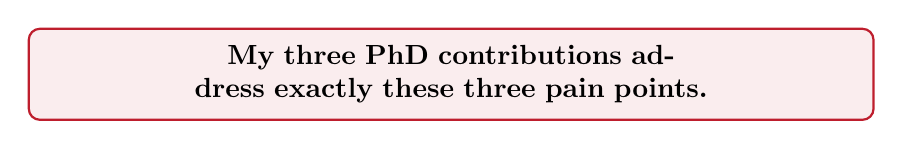
\begin{tikzpicture}
  \node[draw=bellred, thick, rounded corners, fill=bellred!8,
        text width=0.85\linewidth, align=center, inner sep=6pt] {
    \textbf{My three PhD contributions address exactly these three pain points.}
  };
\end{tikzpicture}

\end{frame}

% ============================================================
\section{Contribution 1 — CALASH: Carbon-Aware Lifecycle Routing}
% ============================================================

% ────────────────────────────────────────────────────────────
% SLIDE 5 — CALASH Overview  (~120 s)
% ────────────────────────────────────────────────────────────
\begin{frame}{CALASH — Carbon-Aware Lifecycle-Adaptive Self-Healing Routing}

\begin{columns}[T]
\begin{column}{0.52\textwidth}

  \begin{block}{The Core Insight}
    \vspace{2pt}
    Embodied carbon of one IoT/RAN node $\approx$\textbf{10\,000 gCO\textsubscript{2}eq}\\
    Operational carbon per packet $\approx$\textbf{0.01 gCO\textsubscript{2}eq}\\[4pt]
    $\Rightarrow$ \textbf{Ratio 10\textsuperscript{6}:1} — lifetime extension \textit{is} the carbon strategy.
    \vspace{2pt}
  \end{block}

  \vspace{4pt}
  \textbf{Four integrated pillars:}
  \begin{enumerate}\setlength{\itemsep}{2pt}
    \item \textbf{CADR} — Adaptive compressive sensing ($\rho \!\in\! [0.3, 0.8]$), fidelity $F \!>\! 0.99$
    \item \textbf{CARE} — Lyapunov-DQN carbon-aware router (grid intensity-aware)
    \item \textbf{SHDR} — MAPE-K self-healing (failure tolerance)
    \item \textbf{LSE} — ISO 14040 lifecycle carbon engine (embodied + operational + EoL)
  \end{enumerate}

\end{column}
\begin{column}{0.45\textwidth}

  \begin{alertblock}{Formal Guarantee — CDL Pareto Bound}
    \vspace{2pt}
    For any control parameter $V > 0$, simultaneously:
    \[
      \bar{D} \;\geq\; \bar{D}^* - \frac{B}{V}
      \quad\text{and}\quad
      \bar{C}_{\mathrm{tot}} \;\leq\; \bar{c} + \frac{B}{V}
    \]
    {\small Delivery $\bar{D}$ stays near-optimal \textit{and} carbon $\bar{C}_{\mathrm{tot}}$ stays bounded — \textit{simultaneously}.}
    \vspace{2pt}
  \end{alertblock}

  \vspace{6pt}
  \begin{table}[h]
    \centering
    \scriptsize
    \begin{tabular}{lcc}
      \toprule
      \textbf{Metric} & \textbf{CALASH} & \textbf{Best Baseline}\\
      \midrule
      Network lifetime & \cellcolor{polygreen!20}\textbf{+60\%} & 0\% \\
      Lifecycle carbon (LCI) & \cellcolor{polygreen!20}\textbf{$-33\%$} & $-$8\% \\
      Packet delivery ratio & \textbf{82.9\%} & 79.1\% \\
      Data fidelity ($F$) & \textbf{1.000} & 0.98 \\
      \bottomrule
    \end{tabular}
  \end{table}

\end{column}
\end{columns}

\vspace{2pt}
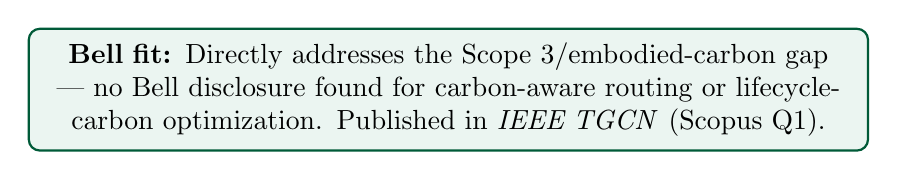
\begin{tikzpicture}
  \node[draw=polygreen!70!black, thick, rounded corners, fill=polygreen!8,
        text width=0.85\linewidth, align=center, inner sep=5pt] {
    \textbf{Bell fit:} Directly addresses the Scope 3/embodied-carbon gap — no Bell disclosure found for carbon-aware routing or lifecycle-carbon optimization. Published in \textit{IEEE TGCN} (Scopus Q1).
  };
\end{tikzpicture}

\end{frame}

% ============================================================
\section{Contribution 2 — CASTER-ZT: Zero-Trust Autonomous Recovery}
% ============================================================

% ────────────────────────────────────────────────────────────
% SLIDE 6 — CASTER-ZT Overview  (~120 s)
% ────────────────────────────────────────────────────────────
\begin{frame}{CASTER-ZT — Zero-Trust Shielded Recovery for Autonomous RAN}

\begin{columns}[T]
\begin{column}{0.52\textwidth}

  \begin{block}{The O-RAN Security Problem}
    \vspace{2pt}
    Open RAN expands the attack surface: open interfaces, multi-vendor xApps,
    AI/ML pipelines, O-Cloud. O-RAN WG11 catalogued
    \textbf{160+ distinct threats} including model poisoning,
    membership inference, and AI supply-chain attacks.\\[4pt]
    Near-RT RIC budget: \textbf{10–1000 ms} — any security guardrail must stay inside.
    \vspace{2pt}
  \end{block}

  \vspace{4pt}
  \textbf{CASTER-ZT 5-stage pipeline:}
  \begin{enumerate}\setlength{\itemsep}{1pt}
    \item \textbf{GNN encoder} — topology-aware state representation
    \item \textbf{Learned recovery policy} — GNN-guided action selection
    \item \textbf{Dual-hypothesis trust–risk evaluator} — Bayesian anomaly scoring
    \item \textbf{MC-Dropout uncertainty} — conformal coverage guarantee (distribution-free)
    \item \textbf{Deterministic formal shield} — 10 proved properties, always-on guardrail
  \end{enumerate}

  \vspace{4pt}
  \textbf{5 graduated decisions:}
  {\small Authorize / Scope-reduce / Defer / Escalate / Block}

\end{column}
\begin{column}{0.45\textwidth}

  \begin{alertblock}{Key Results}
    \vspace{2pt}
    \begin{tabular}{lc}
      \toprule
      \textbf{Metric} & \textbf{Value}\\
      \midrule
      Decision latency & \textbf{3.07 ms} $<$ 10 ms O-RAN budget \\
      Rogue detection (12 cells) & \textbf{74.2\%} @ 0\% FP \\
      Rogue detection (100 cells) & \textbf{98.3\%} @ 0\% FP \\
      Recovery score $\omega_{\mathrm{rec}}$ & \textbf{0.733} vs 0.14–0.20 \\
      Formal properties proved & \textbf{10} \\
      \bottomrule
    \end{tabular}
    \vspace{2pt}
  \end{alertblock}

  \vspace{6pt}
  \begin{exampleblock}{Canadian Regulatory Hook}
    \vspace{2pt}
    \begin{itemize}\setlength{\itemsep}{2pt}
      \item[\textbullet] \textbf{Bill C-8}: critical-infrastructure cyber obligations
      \item[\textbullet] \textbf{CSE Telecoms Cyber Resilience Program}: supply-chain + architecture standards
      \item[\textbullet] \textbf{O-RAN WG11 2026}: AI/ML threat classification now mandatory
    \end{itemize}
    \vspace{2pt}
  \end{exampleblock}

\end{column}
\end{columns}

\vspace{2pt}
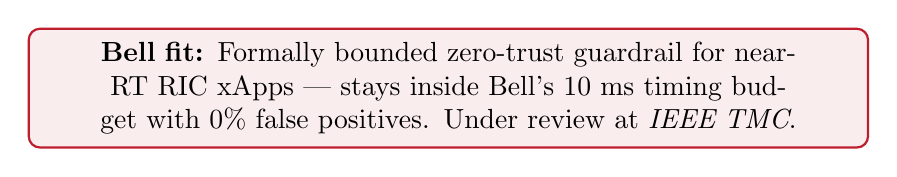
\begin{tikzpicture}
  \node[draw=bellred, thick, rounded corners, fill=bellred!8,
        text width=0.85\linewidth, align=center, inner sep=5pt] {
    \textbf{Bell fit:} Formally bounded zero-trust guardrail for near-RT RIC xApps — stays inside Bell's 10 ms timing budget with 0\% false positives. Under review at \textit{IEEE TMC}.
  };
\end{tikzpicture}

\end{frame}

% ============================================================
\section{Contribution 3 — GAPF: TinyML Autonomous Routing}
% ============================================================

% ────────────────────────────────────────────────────────────
% SLIDE 7 — GAPF Overview  (~90 s)
% ────────────────────────────────────────────────────────────
\begin{frame}{GAPF — TinyML Graph-Attentive Policy Fusion for Rural/IoT Networks}

\begin{columns}[T]
\begin{column}{0.52\textwidth}

  \begin{block}{The Problem: Sub-1W Autonomy at the Edge}
    \vspace{2pt}
    Canada has \textbf{65.7\%} broadband coverage on First Nations reserves.\\
    Bell's public-safety and IoT portfolio requires autonomous,
    battery-powered sensors for \textbf{remote monitoring, NG9-1-1,
    wildfire, and flood sensing}.\\[4pt]
    Existing MARL controllers are too large for constrained hardware ($>$10k parameters).
    \vspace{2pt}
  \end{block}

  \vspace{4pt}
  \textbf{GAPF bi-level architecture:}
  \begin{itemize}\setlength{\itemsep}{2pt}
    \item \textbf{Inner loop} — MARL (QMIX/QTRAN) with\\
          monotonic Q·K attention scalarization\\
          (formally Pareto-guaranteed optimal actions)
    \item \textbf{Outer loop} — Evolution Strategies meta-tuning\\
          of attention weights $\boldsymbol{\alpha}$ (no gradient required)
    \item \textbf{Deployment} — ARM Cortex-M4 / TinyML compatible
  \end{itemize}

\end{column}
\begin{column}{0.45\textwidth}

  \begin{alertblock}{Performance vs.\ Baselines}
    \vspace{2pt}
    \begin{tabular}{lcc}
      \toprule
      \textbf{Metric} & \textbf{GAPF} & \textbf{Best Baseline}\\
      \midrule
      Parameters & \cellcolor{polygreen!20}\textbf{1,473} & 19,200 \\
      Memory reduction & \cellcolor{polygreen!20}\textbf{13$\times$} & — \\
      Energy reduction & \cellcolor{polygreen!20}\textbf{2–3.5$\times$} & — \\
      PDR & \textbf{$\geq$98\%} & 91\% \\
      TinyML (Cortex-M4) & \textbf{\checkmark} & $\times$ \\
      \bottomrule
    \end{tabular}
    \vspace{2pt}
  \end{alertblock}

  \vspace{4pt}
  \begin{exampleblock}{Bell Application Framing}
    \vspace{2pt}
    \begin{itemize}\setlength{\itemsep}{2pt}
      \item[\textbullet] \textbf{Rural/Indigenous sensor mesh}: reduce truck rolls
      \item[\textbullet] \textbf{Bell AI Fabric edge inference}: sub-1W distributed control
      \item[\textbullet] \textbf{NB-IoT / LTE-M} compatible mMTC gateway routing
      \item[\textbullet] \textbf{Public-safety resilient mesh}: disaster monitoring
    \end{itemize}
    \vspace{2pt}
  \end{exampleblock}

\end{column}
\end{columns}

\vspace{2pt}
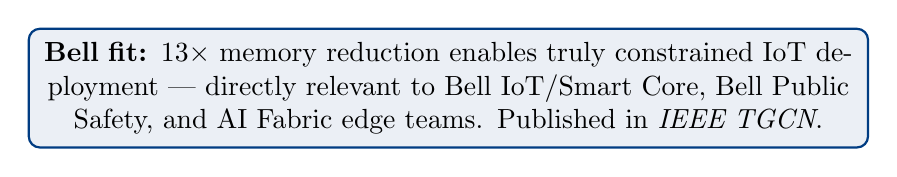
\begin{tikzpicture}
  \node[draw=bellblue, thick, rounded corners, fill=bellblue!8,
        text width=0.85\linewidth, align=center, inner sep=5pt] {
    \textbf{Bell fit:} 13$\times$ memory reduction enables truly constrained IoT deployment — directly relevant to Bell IoT/Smart Core, Bell Public Safety, and AI Fabric edge teams. Published in \textit{IEEE TGCN}.
  };
\end{tikzpicture}

\end{frame}

% ============================================================
\section{Evidence Alignment \& Positioning}
% ============================================================

% ────────────────────────────────────────────────────────────
% SLIDE 8 — Alignment Table  (~60 s)
% ────────────────────────────────────────────────────────────
\begin{frame}{Thesis vs.\ Bell's Confirmed Strategic Priorities}

\centering
\renewcommand{\arraystretch}{1.25}
\scriptsize
\begin{tabularx}{\linewidth}{>{\bfseries}p{3.0cm} X X X}
\toprule
\textbf{Bell Priority} & \textbf{CALASH} & \textbf{CASTER-ZT} & \textbf{GAPF} \\
\midrule
AI-native RAN efficiency & Carbon-aware Lyapunov-DQN routing & GNN-based recovery policy & MARL meta-controller (1,473 params) \\
\addlinespace
Cloud / O-RAN path & CDL Pareto bound for SLA + carbon & ZT shield for xApp/rApp security & Distributed edge control \\
\addlinespace
Network energy (BCE $-58\%$ Scope 1+2) & \cellcolor{polygreen!20}\textbf{Addresses embodied + operational} & $-$ & Reduces active-transmit energy 2–3.5$\times$ \\
\addlinespace
Scope 3 embodied carbon (91\% of footprint) & \cellcolor{polygreen!20}\textbf{ISO 14040 lifecycle engine} & $-$ & Lifetime extension $\Rightarrow$ deferred hardware \\
\addlinespace
O-RAN / near-RT RIC (10 ms budget) & $-$ & \cellcolor{bellred!15}\textbf{3.07 ms, 0\% FP, 10 proved props} & $-$ \\
\addlinespace
Bill C-8 cyber compliance & $-$ & \cellcolor{bellred!15}\textbf{Formally verifiable guardrail} & $-$ \\
\addlinespace
Rural / Indigenous connectivity & $+$ lifetime $\Rightarrow$ fewer replacements & $+$ resilient recovery & \cellcolor{bellblue!15}\textbf{TinyML Cortex-M4, 98\% PDR} \\
\addlinespace
Bell AI Fabric / MEC & Grid-carbon-aware edge offload & Secure xApp deployment & Sub-1W distributed inference \\
\addlinespace
NTN / public safety & Self-healing MAPE-K & Rogue detection in mesh & Disaster-resilient sensor mesh \\
\bottomrule
\end{tabularx}

\vspace{6pt}
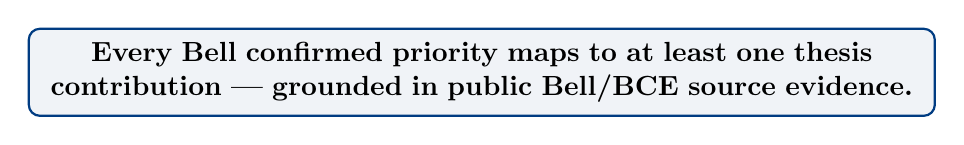
\begin{tikzpicture}
  \node[draw=bellblue, thick, rounded corners, fill=bellblue!6,
        text width=0.92\linewidth, align=center, inner sep=5pt] {
    \textbf{Every Bell confirmed priority maps to at least one thesis contribution — grounded in public Bell/BCE source evidence.}
  };
\end{tikzpicture}

\end{frame}

% ============================================================
\section{Collaboration Proposal \& Ask}
% ============================================================

% ────────────────────────────────────────────────────────────
% SLIDE 9 — Collaboration Proposal  (~90 s)
% ────────────────────────────────────────────────────────────
\begin{frame}{Collaboration Proposal — Three Actionable Pathways}

\begin{columns}[T]

\begin{column}{0.32\textwidth}
  \begin{block}{Pathway A — MITACS}
    \vspace{2pt}
    \textbf{CALASH on Bell IoT/RAN testbed}\\[4pt]
    \begin{itemize}\setlength{\itemsep}{2pt}
      \item[\textbullet] Duration: 6–12 months
      \item[\textbullet] Goal: Validate carbon-aware routing on real NB-IoT/LTE-M traffic and provincial grid-carbon data
      \item[\textbullet] Bell teams: Network Operations, ESG, AI Fabric
      \item[\textbullet] Deliverable: Bell-operable carbon decision module + ISO 14040 audit trail
    \end{itemize}
    \vspace{2pt}
    {\scriptsize Funding: MITACS Accelerate ($\sim$\$15k/6 months)}
  \end{block}
\end{column}

\begin{column}{0.32\textwidth}
  \begin{alertblock}{Pathway B — NSERC CRD}
    \vspace{2pt}
    \textbf{CASTER-ZT O-RAN Security Lab}\\[4pt]
    \begin{itemize}\setlength{\itemsep}{2pt}
      \item[\textbullet] Duration: 2–3 years
      \item[\textbullet] Goal: Hardware-in-the-loop near-RT RIC zero-trust testbed, rogue xApp emulation
      \item[\textbullet] Bell teams: Bell Cyber, Mobility RAN Automation, PSBN
      \item[\textbullet] Deliverable: Open-source ZT-xApp guardrail, threat model for E2/A1/O1/R1
    \end{itemize}
    \vspace{2pt}
    {\scriptsize Funding: NSERC CRD ($\sim$\$75k/year)}
  \end{alertblock}
\end{column}

\begin{column}{0.32\textwidth}
  \begin{exampleblock}{Pathway C — Bell AI Fabric Pilot}
    \vspace{2pt}
    \textbf{GAPF TinyML Edge Deployment}\\[4pt]
    \begin{itemize}\setlength{\itemsep}{2pt}
      \item[\textbullet] Duration: 6 months PoC
      \item[\textbullet] Goal: Deploy GAPF on Cortex-M4 nodes in a rural/Indigenous sensor mesh, measure truck-roll reduction
      \item[\textbullet] Bell teams: Bell IoT, Public Safety, AI Fabric
      \item[\textbullet] Deliverable: TinyML firmware + energy/PDR field measurements
    \end{itemize}
    \vspace{2pt}
    {\scriptsize Funding: Bell Innovation Fund / NSERC Alliance}
  \end{exampleblock}
\end{column}

\end{columns}

\vspace{4pt}
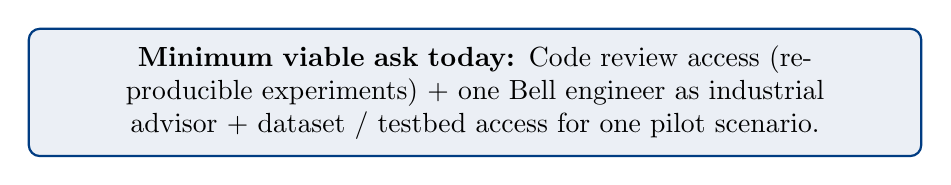
\begin{tikzpicture}
  \node[draw=bellblue, thick, rounded corners, fill=bellblue!8,
        text width=0.90\linewidth, align=center, inner sep=6pt] {
    \textbf{Minimum viable ask today:}
    Code review access (reproducible experiments) $+$ one Bell engineer as industrial advisor $+$ dataset / testbed access for one pilot scenario.
  };
\end{tikzpicture}

\end{frame}

% ────────────────────────────────────────────────────────────
% SLIDE 10 — Closing  (~30 s)
% ────────────────────────────────────────────────────────────
\begin{frame}{Closing Statement}

\vspace{0.5cm}
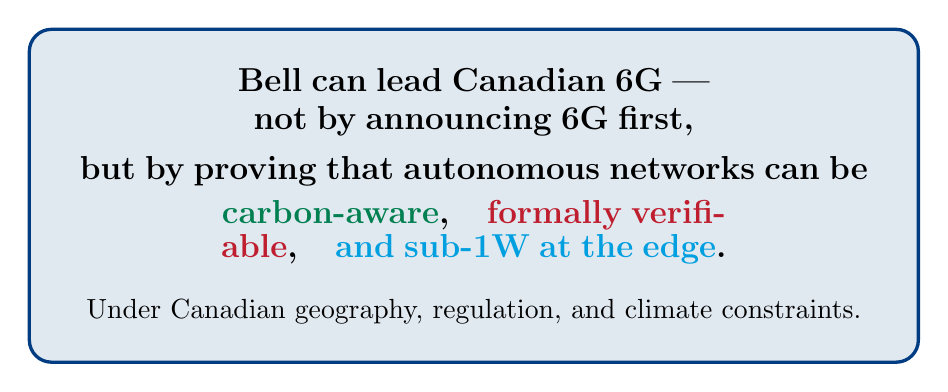
\begin{tikzpicture}
  \node[draw=bellblue, very thick, rounded corners=8pt,
        fill=bellblue!12, text width=0.85\linewidth, align=center, inner sep=14pt] {
    {\large\textbf{Bell can lead Canadian 6G — not by announcing 6G first,\\[4pt]
    but by proving that autonomous networks can be\\[4pt]
    \textcolor{polygreen}{\textbf{carbon-aware}},\quad
    \textcolor{bellred}{\textbf{formally verifiable}},\quad
    \textcolor{polylightblue}{\textbf{and sub-1W at the edge}}.}}\\[10pt]
    {\normalsize Under Canadian geography, regulation, and climate constraints.}
  };
\end{tikzpicture}

\vspace{0.6cm}

\begin{columns}[c]
\begin{column}{0.33\textwidth}
  \centering
  \begin{block}{\centering Publications}
    \scriptsize
    \textit{IEEE TGCN} (Scopus Q1) \\
    GAPF + CALASH accepted\\[2pt]
    \textit{IEEE TMC} (under review)\\
    CASTER-ZT
  \end{block}
\end{column}
\begin{column}{0.33\textwidth}
  \centering
  \begin{block}{\centering Code \& Reproducibility}
    \scriptsize
    Open-source repositories\\
    All experiments reproducible\\
    Python + PyTorch + formal proofs\\
    Available for Bell review
  \end{block}
\end{column}
\begin{column}{0.33\textwidth}
  \centering
  \begin{block}{\centering Contact}
    \scriptsize
    \textbf{Georges Parfait Djimefo Kapen}\\
    PhD Candidate, LARIM\\
    Polytechnique Montréal\\
    {\footnotesize\texttt{djimefokapen@polymtl.ca}}
  \end{block}
\end{column}
\end{columns}

\vspace{0.3cm}
\centering
\textcolor{bellgray}{\small \textit{Thank you — questions welcome.}}

\end{frame}

% ============================================================
%  APPENDIX — Backup slides
% ============================================================
\appendix

% ────────────────────────────────────────────────────────────
% BACKUP A — CALASH Lyapunov derivation
% ────────────────────────────────────────────────────────────
\begin{frame}[label=backup-calash]{Backup — CALASH: CDL Theorem (Proof Sketch)}

  \begin{block}{Virtual Queue $Z(t)$ and Lyapunov Drift-Plus-Penalty}
    \vspace{2pt}
    Define virtual carbon queue:
    $Z(t+1) = \max\bigl[Z(t) + C_t - \bar{c},\; 0\bigr]$\\
    Lyapunov function: $L(t) = \tfrac{1}{2}Z(t)^2$\\[4pt]
    Minimize per-slot drift-plus-penalty:
    $\Delta L(t) + V \cdot C_t^{\mathrm{total}} - V \cdot \lambda \cdot D_t$\\[4pt]
    Under standard Lyapunov stability analysis, the time-average:
    \[
      \bar{D} \geq \bar{D}^* - \frac{B}{V}
      \quad\text{and}\quad
      \bar{C}_{\mathrm{tot}} \leq \bar{c} + \frac{B}{V}
    \]
    hold simultaneously for any $V > 0$, where $B$ is a finite constant.
    \vspace{2pt}
  \end{block}

  \textbf{Interpretation:} Increasing $V$ trades smaller carbon slack for better delivery optimality. The Pareto front is convex and fully traceable by varying a single scalar.

\end{frame}

% ────────────────────────────────────────────────────────────
% BACKUP B — CASTER-ZT 10 formal properties
% ────────────────────────────────────────────────────────────
\begin{frame}[label=backup-caster]{Backup — CASTER-ZT: 10 Proved Formal Properties}

\begin{columns}[T]
\begin{column}{0.48\textwidth}
  \begin{enumerate}\setlength{\itemsep}{2pt}
    \item \textbf{Safety:} No unsafe action admitted by the shield
    \item \textbf{Liveness:} Recovery is always eventually initiated
    \item \textbf{Bounded admissibility:} Only actions within policy envelope admitted
    \item \textbf{Rogue isolation:} Rogue agents cannot influence quorum decisions
    \item \textbf{False-positive bound:} FP rate $\leq \delta$ (conformal coverage)
  \end{enumerate}
\end{column}
\begin{column}{0.48\textwidth}
  \begin{enumerate}\setlength{\itemsep}{2pt}
    \setcounter{enumi}{5}
    \item \textbf{Timing compliance:} Decision latency $< 10$ ms budget
    \item \textbf{Conformal coverage:} Distribution-free coverage guarantee
    \item \textbf{Calibration convergence:} MC-Dropout calibration error $\to 0$
    \item \textbf{CDL defense-in-depth:} 5 layers (detect / scope-reduce / defer / escalate / block)
    \item \textbf{Model integrity:} GNN encoder invariant to permutation and node dropout
  \end{enumerate}
\end{column}
\end{columns}

\vspace{4pt}
\textbf{Proof method:} Formal induction on the shield transition system + conformal prediction theory + Lyapunov stability for recovery convergence.

\end{frame}

% ────────────────────────────────────────────────────────────
% BACKUP C — Bell vs. TELUS vs. Rogers comparison
% ────────────────────────────────────────────────────────────
\begin{frame}[label=backup-carriers]{Backup — Canadian Carrier Comparison (6G-Adjacent)}

\centering
\renewcommand{\arraystretch}{1.3}
\scriptsize
\begin{tabularx}{\linewidth}{>{\bfseries}p{3.2cm} X X X}
\toprule
\textbf{Dimension} & \textbf{Bell Mobility} & \textbf{Rogers} & \textbf{TELUS} \\
\midrule
AI-native RAN & \cellcolor{polygreen!20}Strongest: Ericsson live field test (+20\% DL, Apr 2025) & 5G SA + RedCap, less AI-RAN differentiation & AI-RIC via Samsung CognitiV NOS \\
O-RAN / RIC maturity & Cloud RAN (Nokia), no public near-RT RIC & Cloud RAN trial (live event), no commercial O-RAN & \cellcolor{polygreen!20}Canada's 1st commercial vRAN/O-RAN + AI-RIC (Samsung) \\
MEC / edge & \cellcolor{polygreen!20}Leads: AWS Wavelength + Google DCE + AI Fabric & Less public MEC evidence & Sovereign AI factory, strong but Bell leads MEC \\
Sustainability & Strong ESG targets, \textit{no carbon-aware routing} & CTDA participant & Strong brand, Bell stronger on AI-RAN energy \\
Security / ZT & Strong cyber business, \textit{no public O-RAN ZTA} & Post-outage resiliency focus & Signs Global Coalition on 6G Security; stronger O-RAN security visibility \\
6G PHY research & Cohere/OTFS via Bell Ventures, NTN/AST & Limited public 6G PHY work & Limited public 6G PHY work \\
\bottomrule
\end{tabularx}

\vspace{4pt}
{\footnotesize\textit{Sources: Ericsson press release Apr 2025; Nokia MWC 2025; Samsung/TELUS announcements 2024–2025; BCE 2024 Annual Financial Report.}}

\end{frame}

% ────────────────────────────────────────────────────────────
% BACKUP D — Readiness checklist for Bell collaboration
% ────────────────────────────────────────────────────────────
\begin{frame}[label=backup-readiness]{Backup — What Bell Would Need Before Collaboration}

\centering
\renewcommand{\arraystretch}{1.25}
\scriptsize
\begin{tabularx}{\linewidth}{>{\bfseries}p{3.5cm} X X X}
\toprule
\textbf{Requirement} & \textbf{CALASH} & \textbf{CASTER-ZT} & \textbf{GAPF} \\
\midrule
Reproducible code + data & \checkmark Available & \checkmark Available & \checkmark Available \\
Hardware-in-loop demo & Sensor/edge device energy test & O-RAN near-RT security testbed & Cortex-M4 IoT node test \\
Telecom scenario mapping & Provincial grid-carbon $+$ NB-IoT/LTE-M SLA & E2/A1/O1/R1 threat model, rogue xApp emulation & LTE-M / NB-IoT / mMTC traffic \\
Baseline comparisons & Always-active, always-passive, energy-only routing & ZTA detectors, rule-based recovery & RPL, LEACH, MARL/GNN, TinyML \\
Formal due diligence & ISO 14040 assumptions, LCA database & 10 formal proofs, adversarial ML stress-test & Energy + latency on real hardware \\
Deployment pathway & MITACS Accelerate & NSERC CRD & Bell Innovation Fund / NSERC Alliance \\
\bottomrule
\end{tabularx}

\vspace{4pt}
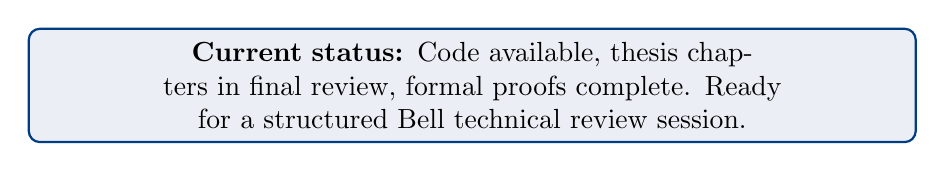
\begin{tikzpicture}
  \node[draw=bellblue, thick, rounded corners, fill=bellblue!8,
        text width=0.90\linewidth, align=center, inner sep=5pt] {
    \textbf{Current status:} Code available, thesis chapters in final review, formal proofs complete. Ready for a structured Bell technical review session.
  };
\end{tikzpicture}

\end{frame}

\end{document}
